\section{ИССЛЕДОВАНИЕ РАБОТЫ МУЛЬТИПЛЕКСОРА}

\begin{figure}[H]
	\centering
	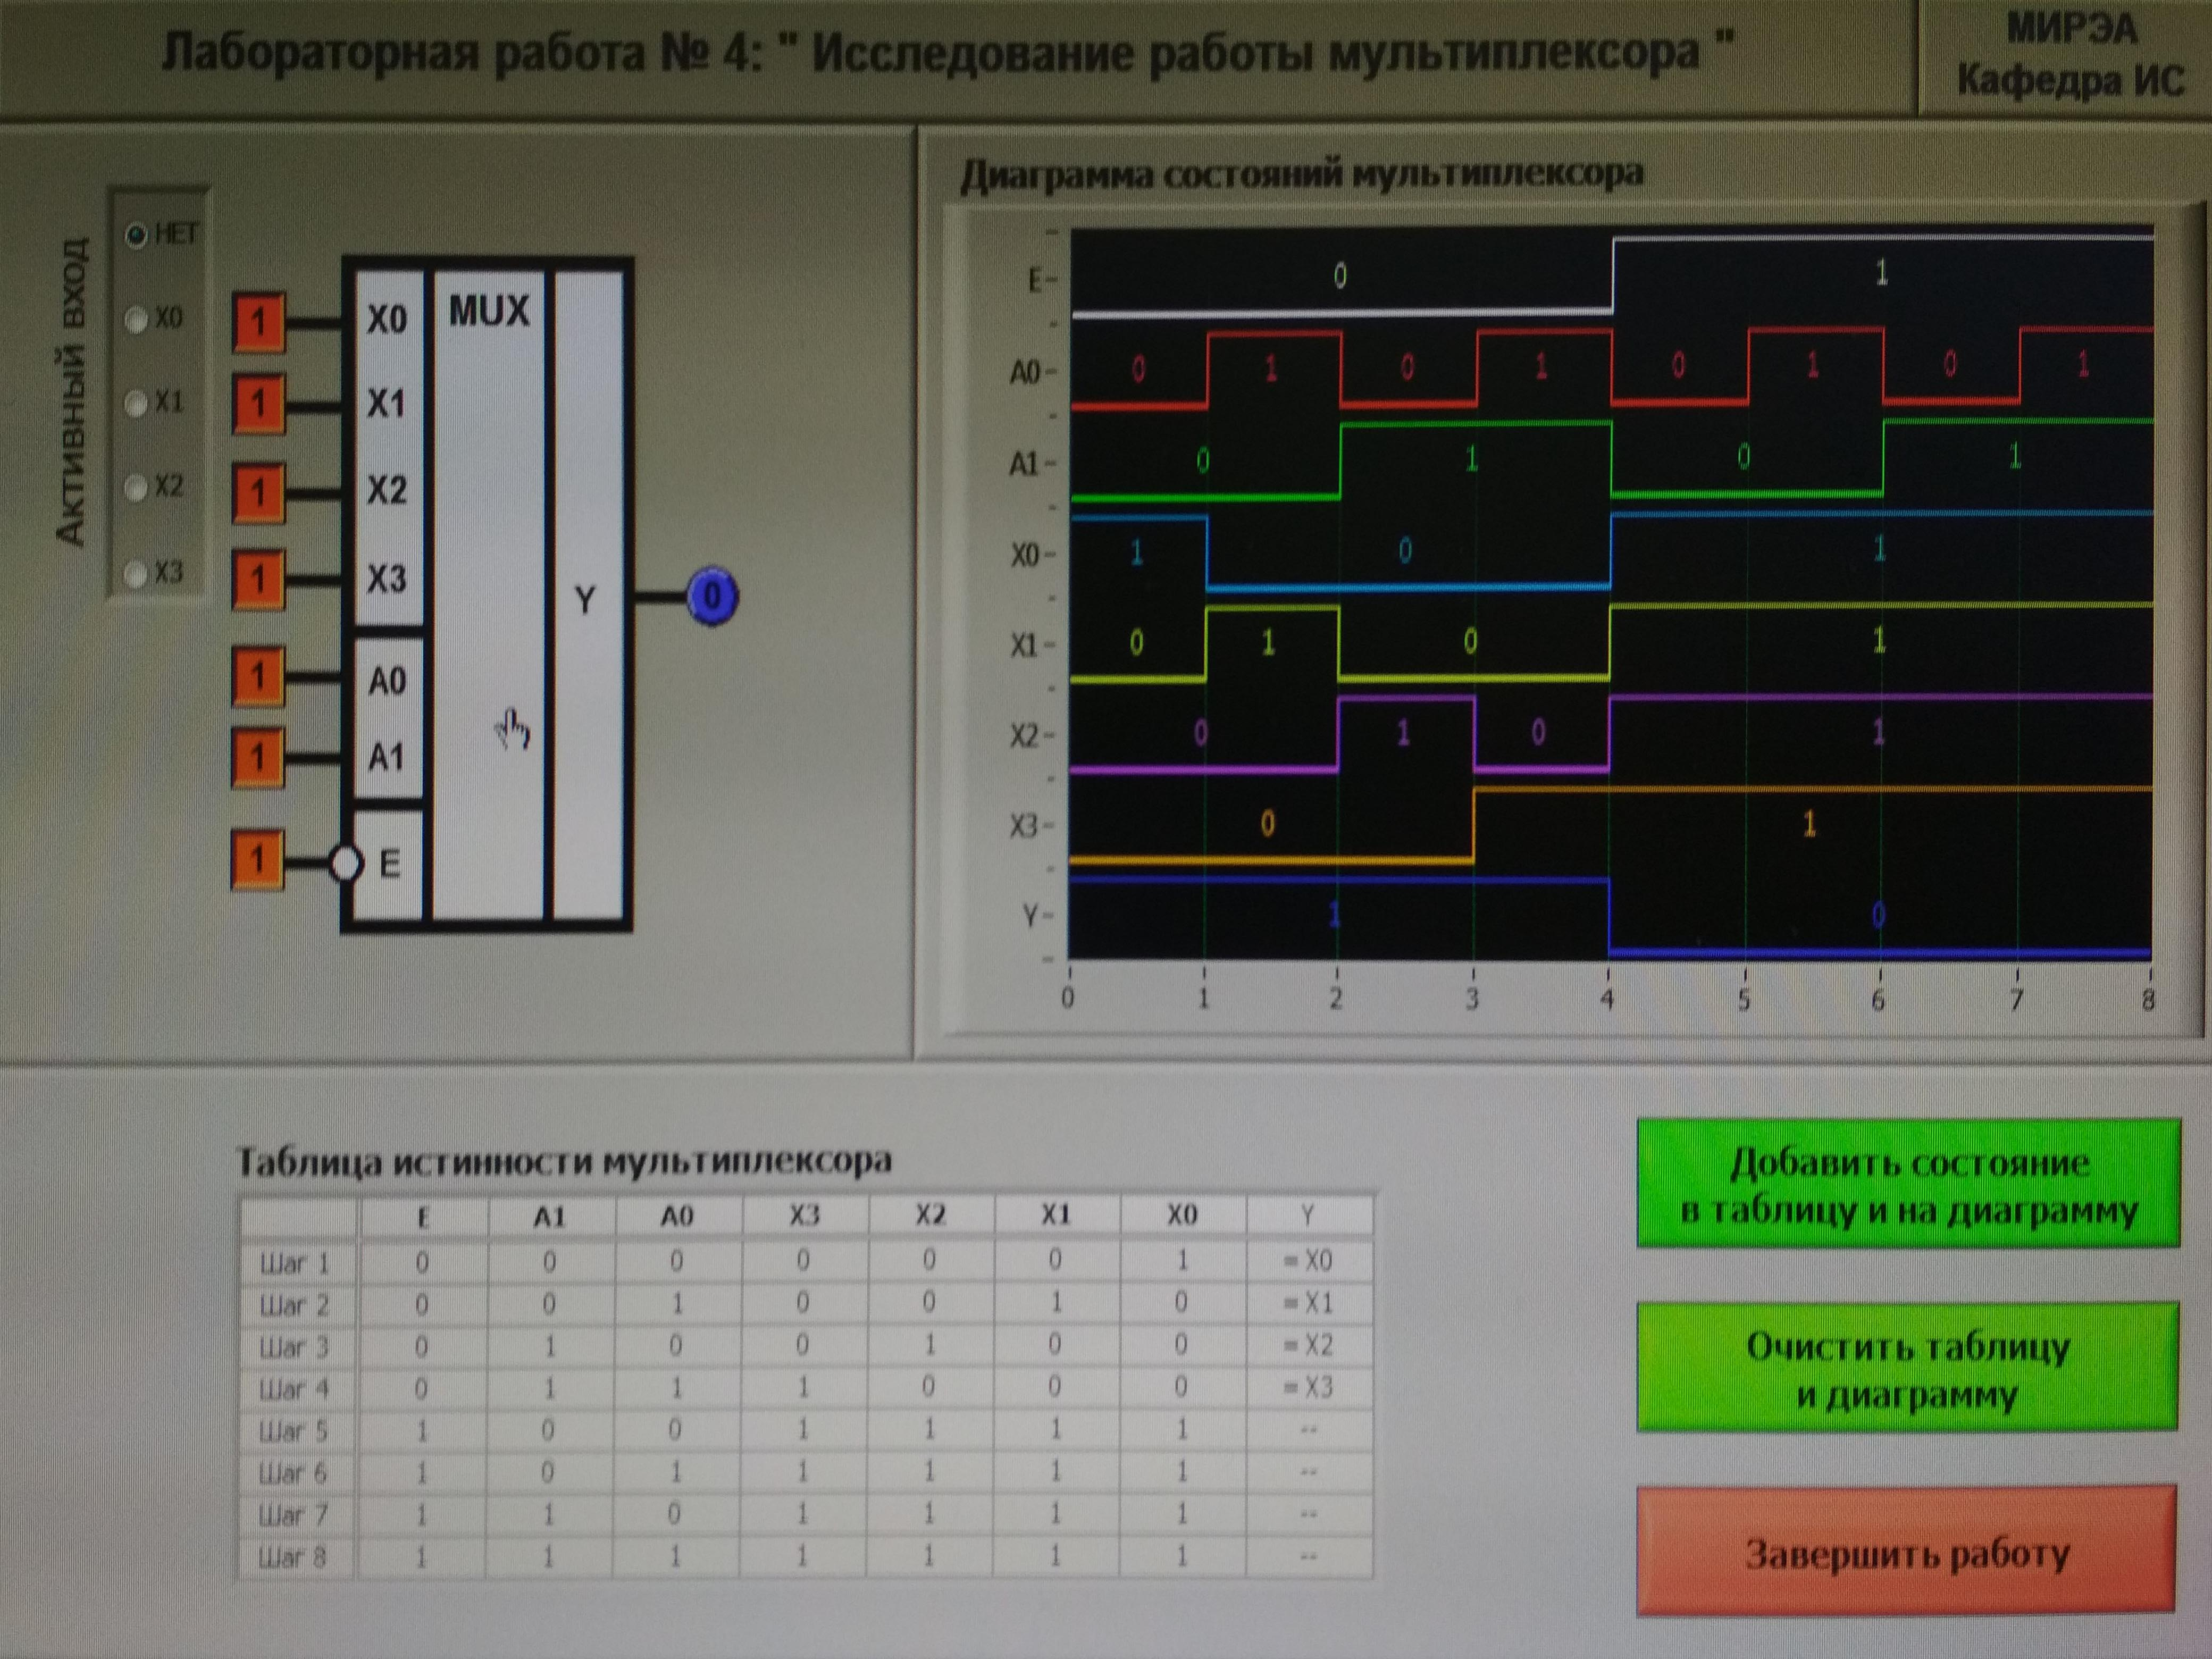
\includegraphics[width=0.95\linewidth]{imgs/4/1}
	\caption{Результат работы мультиплексора}
	\label{fig:4_}
\end{figure}

В ходе работы было выяснено, что для работы дешифратора необходимо подать низкий уровень на вход E.
% Шифратор является приоритетным, вход X6 имеет больший приоритет, чем X3

Элемент SN74LV4052A - CMOS

Характеристики:

\begin{figure}[H]
	\centering
	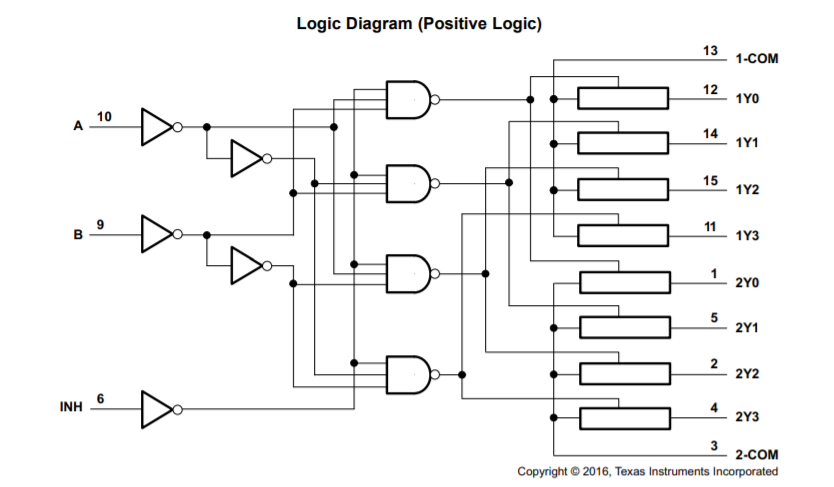
\includegraphics[width=0.95\linewidth]{imgs/4/ti1}
	\caption{Схема}
	\label{fig:4_ti1}
\end{figure}

\begin{figure}[H]
	\centering
	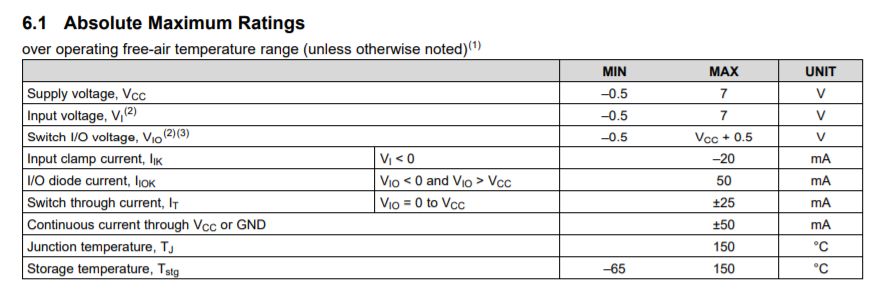
\includegraphics[width=0.95\linewidth]{imgs/4/ti2}
	\caption{Максимальные рабочие параметры}
	\label{fig:4_ti2}
\end{figure}

\begin{figure}[H]
	\centering
	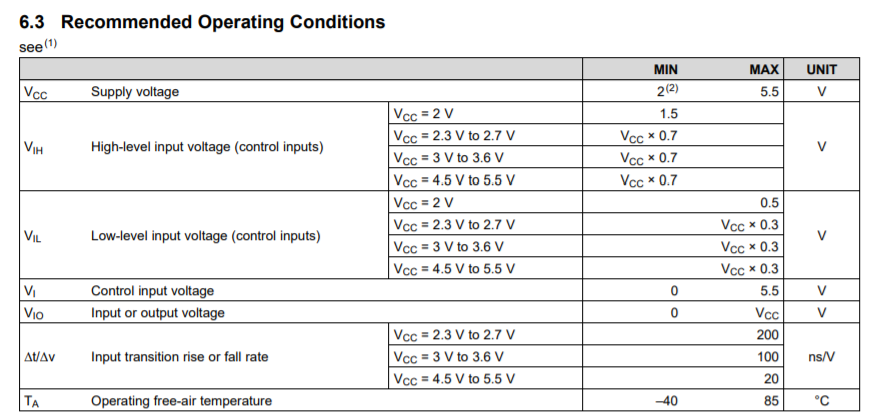
\includegraphics[width=0.95\linewidth]{imgs/4/ti3}
	\caption{Рекомендуемые рабочие параметры}
	\label{fig:4_ti3}
\end{figure}

\begin{figure}[H]
	\centering
	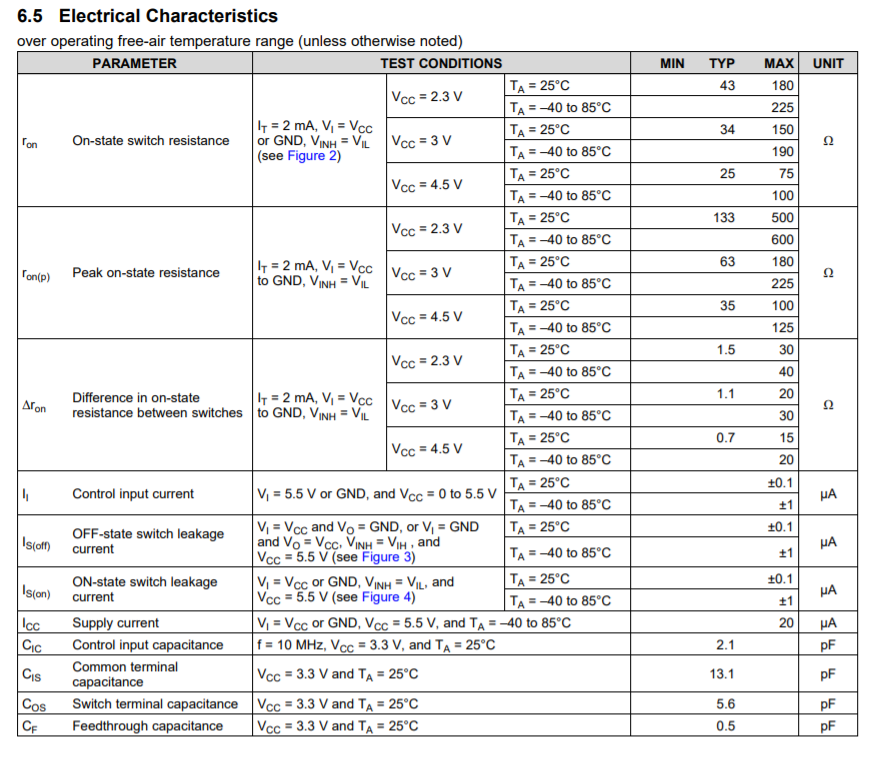
\includegraphics[width=0.95\linewidth]{imgs/4/ti4}
	\caption{Электрические характеристики}
	\label{fig:4_ti4}
\end{figure}